\subsection{Modelos Regressivos}\label{subsec:reg}

Os modelos regressivos para séries temporais são os mais populares na literatura no momento, com base no gradiente. Esses modelos, além do LR simples, são os modelos mais famosos na competição de séries temporais em todo o mundo. 

\subsubsection{Regress\~ao Linear (LR)}

Segundo \citeonline{korstanje2021} nos modelos de aprendizado de máquina supervisionados, você tenta identificar relações entre diferentes variáveis:

\begin{itemize}
	\item Variável de destino: a variável que você tenta prever
	\item Variáveis explicativas: Variáveis que ajudam você a prever o alvo variável
\end{itemize}

Para a previsão, é importante entender quais tipos de variáveis explicativas você pode ou não usar. Como exemplo, aqui vai ser usado as variáveis \textbf{Pressão de Succção (PT01SU)} como variável $x$ e \textbf{Nível do Reservatório (Câmara 1) LT01} como variável $y$ pois na correlação de Pearson mostrado na Figura \ref{fig:person}, o coeficiente mostra a relação que tem entre o eixo $x$ e $y$ com a seguinte fórmula.



\begin{eqnarray}
	r=\frac{\sum\left(x_i-\bar{x}\right)\left(y_i-\bar{y}\right)}{\sqrt{\left(\sum\left(x_i-\bar{x}\right)^2\right)\left(\sum\left(y_i-\bar{y}\right)^2\right)}}\label{eq:pearson}
\end{eqnarray}
De \eqref{eq:pearson} sejam $x_i \in y_i$ os valores das variáveis $X$ e $Y$.  $\bar{x}$ e $\bar{y}$ são respectivamente as médias dos valores $x_i \in y_i$.

A fórmula do coeficiente de correlação de Pearson é então,

\begin{figure}[H]
	\centering
	\caption{Corelação de Pearson}
	\label{fig:person}
	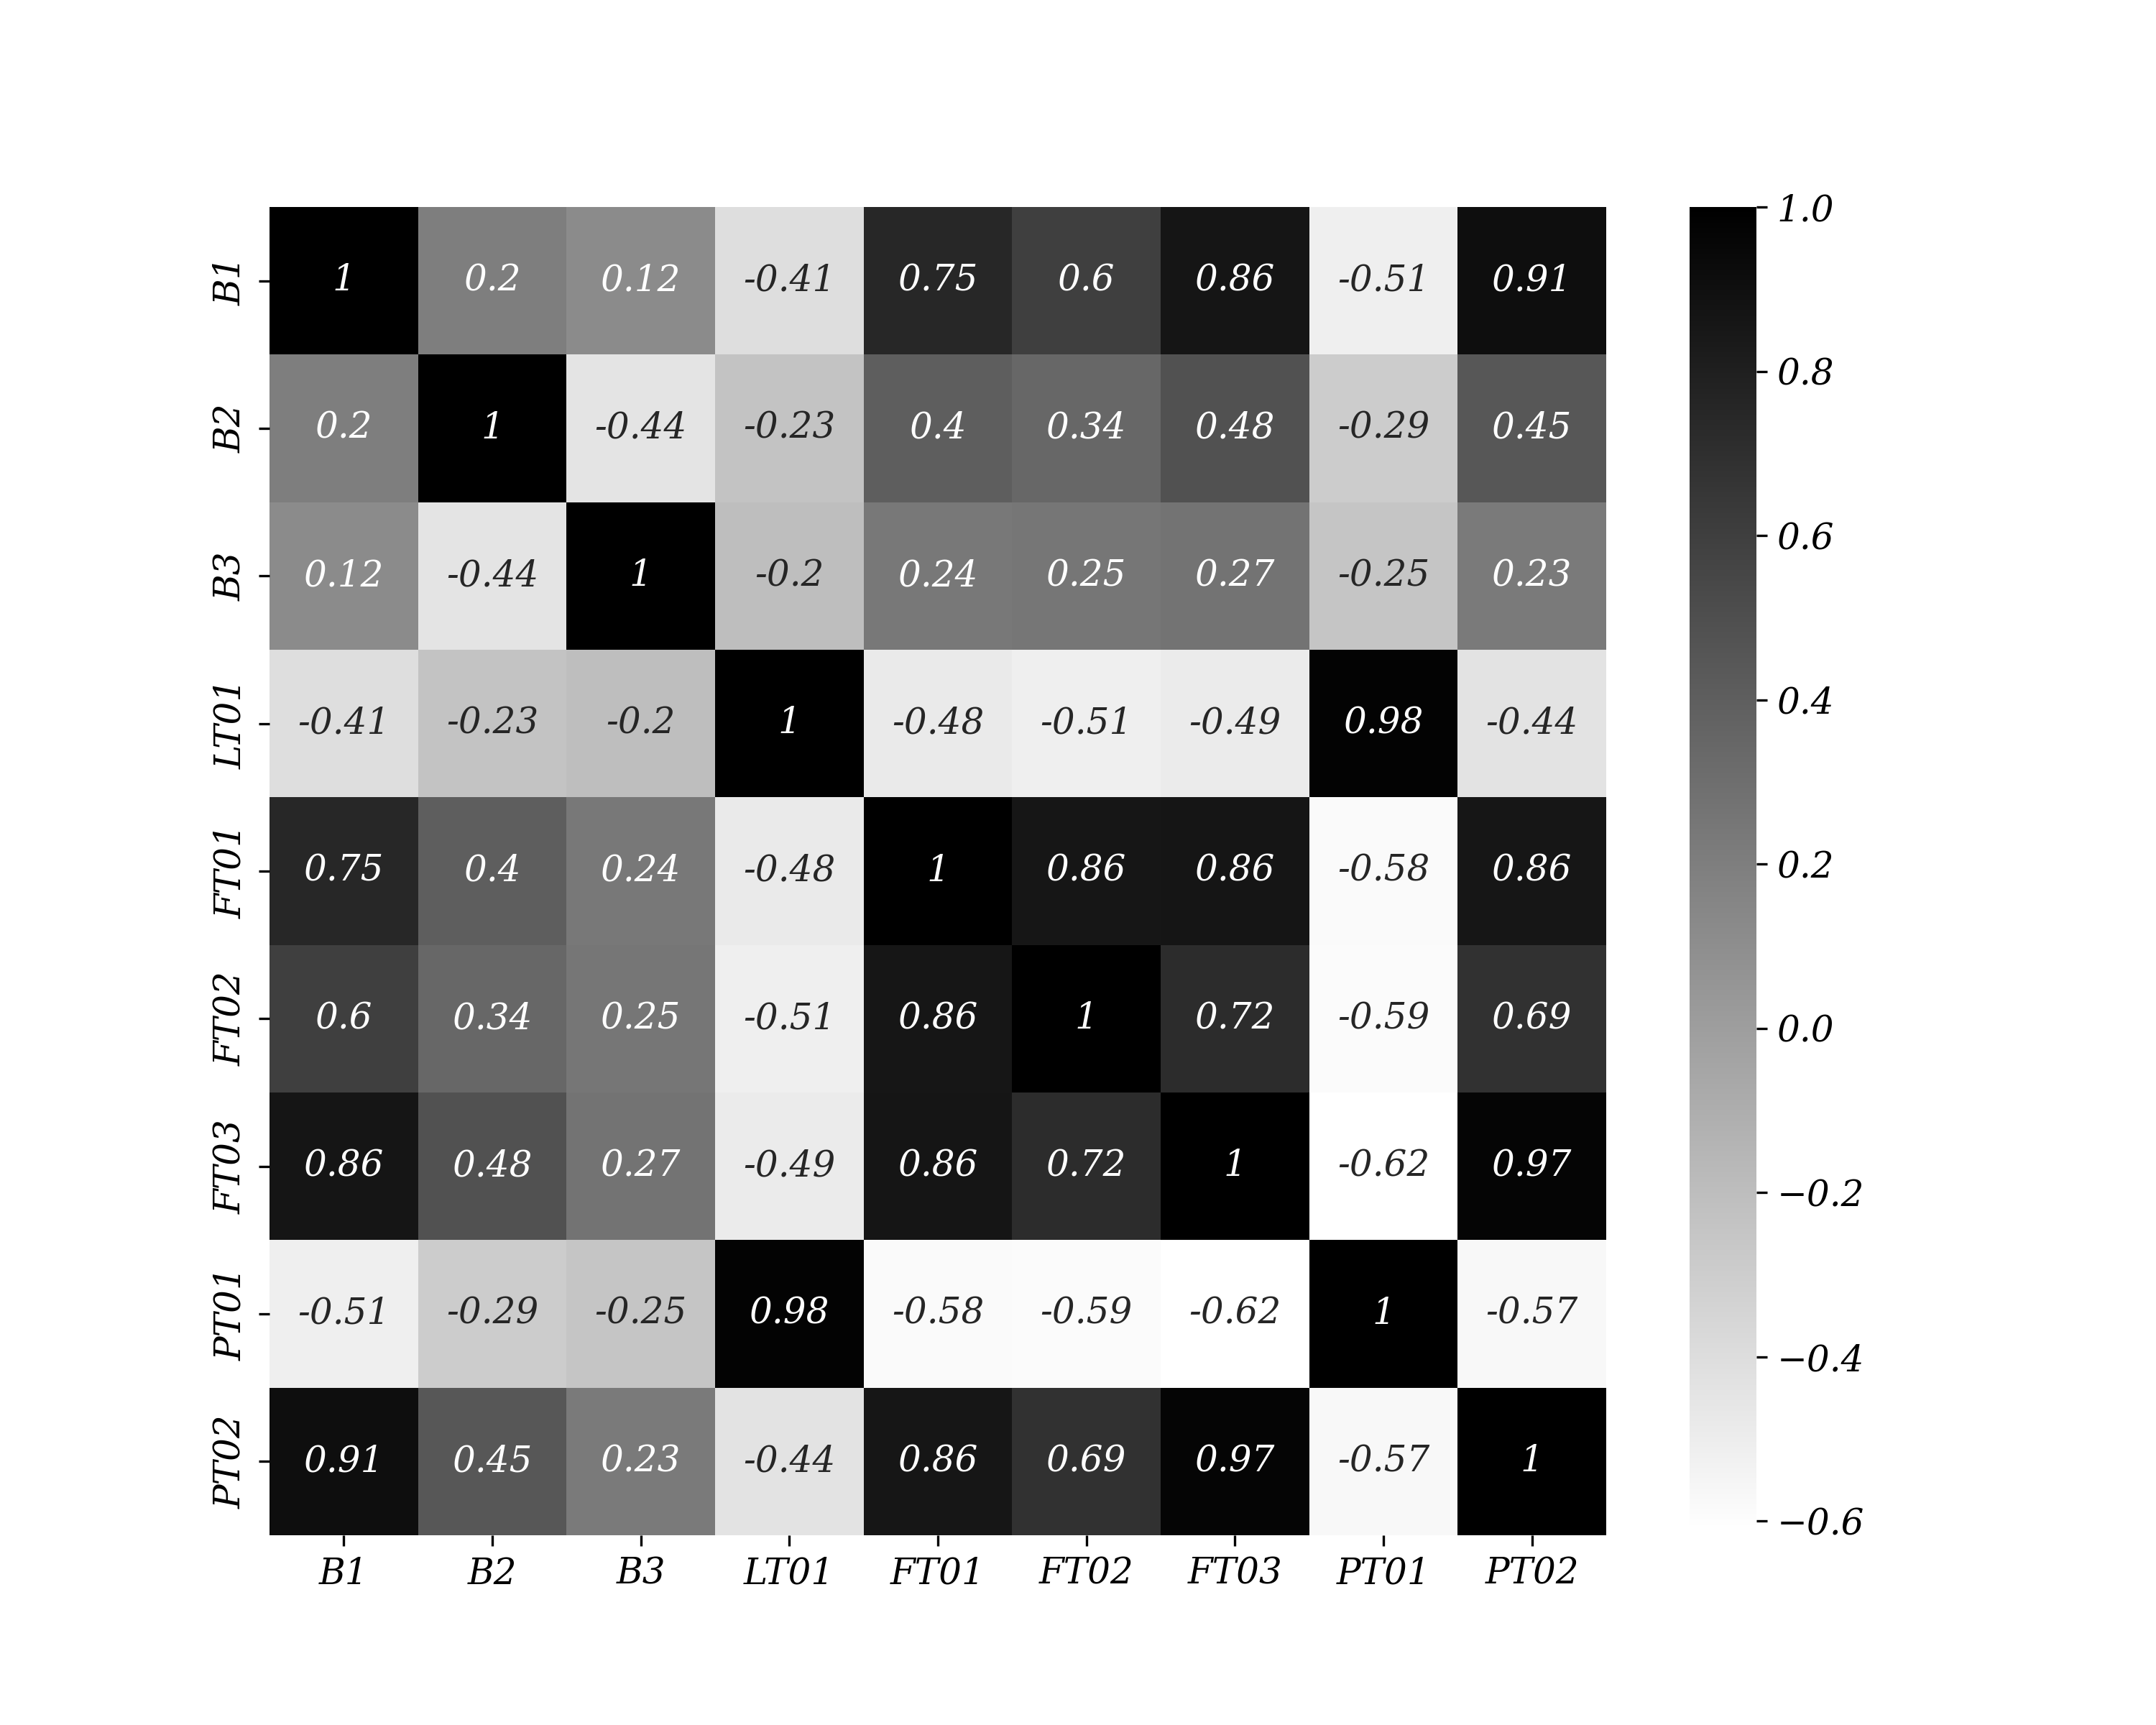
\includegraphics[width=0.7\linewidth]{Apendices/Figuras/modelagem-24h/person}
	
	Fonte: Elaboração própria a partir de dados da SANEPAR (2018 a 2020)
\end{figure}

Como mostra a Figura \ref{fig:person} essa imagem é meramente ilutação da correlação que tem relação no conjunto de dados que esta sendo trabalhado aqui. E com isso também pode ser respondido a \ref{q1} da pesquisa. porque a correlação entre essas variáveis é forte.

\subsubsection{Defini\c c\~ ao do modelo}

A regressão linear é definida da seguinte forma:
\begin{eqnarray}
	y&=&\beta_0+\beta_1 x_1+\cdots+\beta_p x_p+\varepsilon\label{eq:lr}
\end{eqnarray}
Da \eqref{eq:lr} têm a seguinte variáveis:

\begin{itemize}
	\item  Há $p$ variáveis explicativas, chamadas $x$.
	\item Existe uma variável alvo chamada $y$.
	\item  O valor para $y$ é calculado como uma constante $\left(\beta_0\right)$ mais os valores do $x$ variáveis multiplicadas pelos seus coeficientes $\beta_1$ para $\beta_p$.
\end{itemize}

\begin{figure}[H]
	\centering
	\caption{Regressão linear LT01 vs PT01 correlação 98\%}
	\label{fig:lr-lt01-m3}
	\includegraphics[width=0.9\linewidth]{"Modelos/Figuras/LR LT01 (m³)"}
	
	Fonte: Elaboração própria a partir de dados da SANEPAR (2018 a 2020)
\end{figure}



A Figura \ref{fig:lr-lt01-m3} mostra como interpretar $\beta_0$ e $\beta_1$ visualmente. Mostra que para um aumento de $1$ na variável $x$, o aumento na variável $x$ representa $\beta_1$. O valor para $0$ é o valor para $x$ quando $y$ é $0$.

Para poder utilizar a regressão linear, é necessário estimar os coeficientes (betas) sobre um conjunto de dados de formação. Os coeficientes podem então ser estimados utilizando a seguinte fórmula, em notação matricial:

\begin{eqnarray}
	\hat{\beta}&=&\left(X^T X\right)^{-1} X^T y\label{eq:ols}
\end{eqnarray}

\citeonline{korstanje2021} esta fórmula é conhecida como \textbf{OLS}: o método dos mínimos quadrados ordinários (Ordinary Least Squares method). Este modelo é muito rápido para caber, uma vez que requer apenas cálculos matriciais para calcular os betas. Embora fácil para caber, é menos adequado para processos mais complexos. Afinal de contas, é um modelo linear, e pode portanto, só se encaixam em processos lineares.

\begin{figure}[H]
	\centering
	\caption{Regressão linear (LR) um passo a frente}
	\label{fig:1-regressao-linear}
	\includegraphics[width=0.9\linewidth]{Modelos/Figuras/0-regressão-linear}
	
	Fonte: Elaboração própria a partir de dados da SANEPAR (2018 a 2020)
\end{figure}


\subsubsection{Floresta Aleat\'oria} \label{subsubsec:rf}

Pode entender que ter exatamente a mesma árvore de decisão 1000 vezes não tem valor agregado do que usar essa árvore de decisão apenas uma vez.  Em um modelo de conjunto, cada modelo individual deve ser ligeiramente diferente do outro. Existem dois métodos bem conhecidos de criação de coleções: ensacamento e reforço.  Floresta aleatória usa ensacamento para criar um conjunto de árvores de decisão.
\vspace{-5mm}

\begin{figure}[H]
	\centering
	\caption{Regressão da Floresta Aleatória (RFR)}
	\label{fig:1-regressao-rfa}
	\includegraphics[width=0.9\linewidth]{Modelos/Figuras/0-regressão-rfa}
	
	Fonte: Elaboração própria a partir de dados da SANEPAR (2018 a 2020)
\end{figure}

Segundo \citeonline{Pelletier2016156} Cada árvore é construída executando um algoritmo de aprendizado individual que divide o conjunto de variáveis de entrada em subconjuntos com base em um teste de valor de atributo (por exemplo, o coeficiente de Gini). Ao contrário das árvores de decisão (DT) clássicas, as árvores de RFR são construídas sem poda e selecionando aleatoriamente em cada nó um subconjunto de variáveis de entrada. Atualmente, esse número de variáveis utilizadas para dividir um nó de RFR (denotado por $m$) corresponde à raiz quadrada do número de variáveis de entrada.

\begin{figure}[H]
	\centering
	\caption{Esquema da Floresta Aleatória}
	\label{fig:rf}
	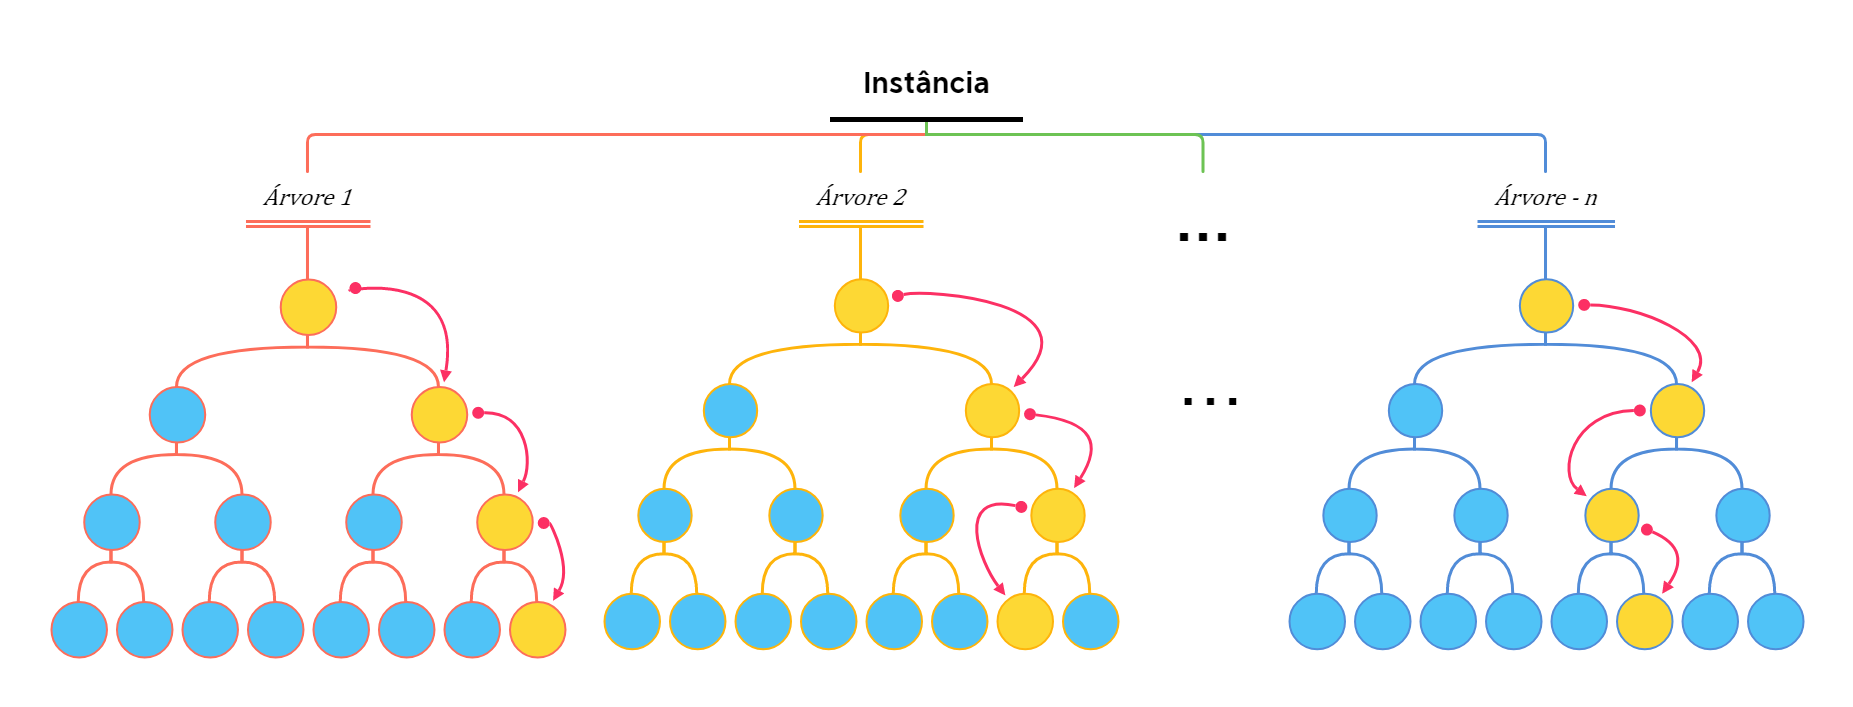
\includegraphics[width=0.9\linewidth]{Modelos/Figuras/RF}
	
	Fonte: Elaboração própria
\end{figure}


\subsubsection{LightGBM e XGboost}\label{subsubsec:lgbxgb}

O aumento de gradiente combina vários pequenos modelos de árvore de decisão para fazer previsões. É claro que essas pequenas árvores de decisão são diferentes umas das outras, caso contrário não há vantagem em usar mais árvores de decisão. O conceito importante a ser entendido aqui é como essas árvores de decisão se tornam diferentes umas das outras. outros. Isto é conseguido através de um processo chamado elevação. Boosting e bagging são dois métodos principais que são aprendidos juntos.  Boosting é um processo iterativo. Ele adiciona cada vez mais modelos fracos ao conjunto de modelos de maneira inteligente. Em cada etapa, pontos de dados individuais são ponderados.  

Pontos de dados que já estão bem previstos não são importantes para o aluno adicionar. Portanto, novos modelos fracos se concentrarão em aprender coisas que ainda não são compreendidas, melhorando assim o conjunto.

Pode se ver uma visão geral esquemática do processo de reforço na Figura \ref{fig:xgboos}. Com essa abordagem, você ajusta iterativamente modelos fracos que se concentram nas partes dos dados que ainda
não são compreendidas. Ao fazer isso, você mantém todos os modelos fracos intermediários. O modelo ensemble é a combinação de todos esses modelos fracos.


\begin{figure}[H]
	\centering
	\caption{Impulsionando gradiente com XGBoost e LightGBM}
	\label{fig:xgboos}
	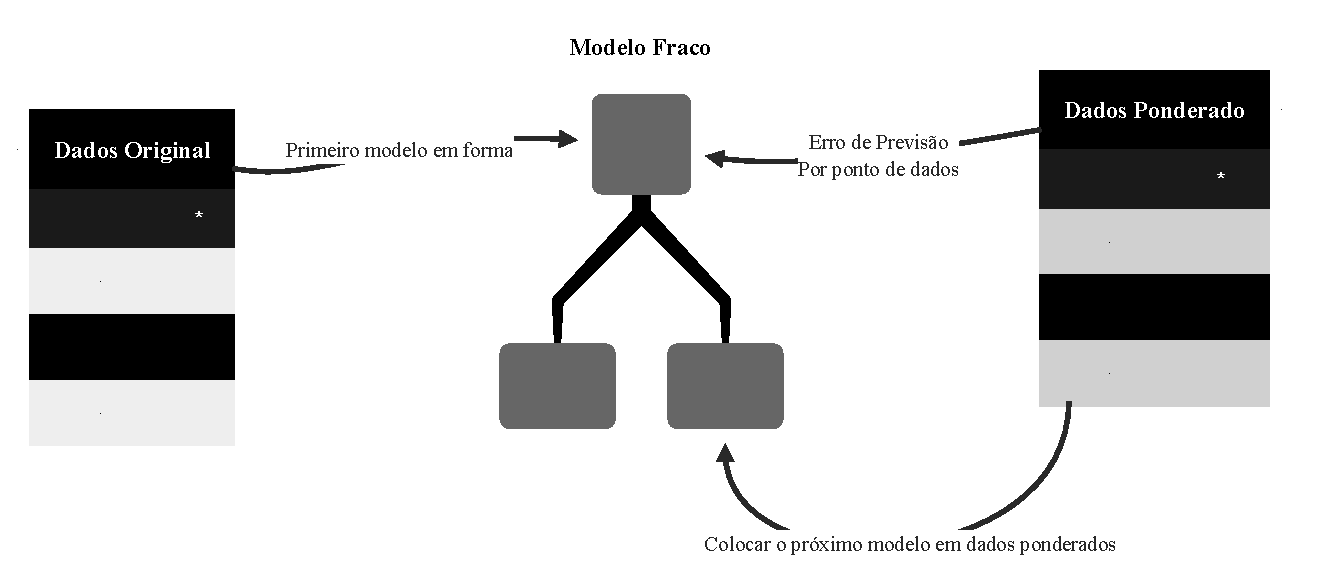
\includegraphics[width=0.9\linewidth]{Modelos/Figuras/xgboos}
	
	Fonte: Adaptação de \citeonline{korstanje2021}
\end{figure}



\subsubsection{O Gradiente em Gradiente de Boosting (Refor\c co)} \label{subsubsec:boosting}

\citeonline{korstanje2021} esse processo iterativo é chamado de aumento de gradiente por um motivo. Um gradiente é um termo matemático que se refere ao campo vetorial de derivadas parciais que apontam na direção da inclinação mais acentuada. Em termos simples, muitas vezes comparamos gradientes com declives de estradas em aclive: quanto maior a inclinação, mais íngreme a colina. Os gradientes são calculados tomando derivadas, ou derivadas parciais, de uma função.

No aumento de gradiente, ao adicionar árvores adicionais ao modelo, o objetivo é adicionar uma árvore que melhor explique a variação que não foi explicada pelas árvores anteriores. O destino de sua nova árvore é, portanto.

\begin{eqnarray}
	y-\hat{y}\label{eq:xb}
\end{eqnarray}

De \eqref{eq:xb} isso pode ser denotado reescrito como a derivada parcial negativa da função de perda em relação às previsões de $y$:

\begin{eqnarray}
	y-\hat{y}&=&-\dfrac{\partial L}{\partial \hat{y}}\label{eq:xb2}
\end{eqnarray}

Você define isso como o destino da nova árvore para garantir que a adição da árvore explicará uma quantidade máxima de variação adicional no modelo geral de aumento de gradiente. Isso explica por que o modelo é chamado de aumento de gradiente boosting.

\subsubsection{Algoritmos de boosting de gradiente}

Existem muitos algoritmos que executam versões ligeiramente diferentes de aumento de gradiente. Quando o método de aumento de gradiente foi inventado, o algoritmo não Muito desempenho, mas mudou com o advento do algoritmo AdaBoost: o primeiro algoritmo que pode se adaptar a modelos fracos. 

O algoritmo de aumento de gradiente é uma das ferramentas de aprendizado de máquina com melhor desempenho no mercado. Depois do AdaBoost, uma longa lista de algoritmos de aumento ligeiramente diferentes foi adicionada à literatura, incluindo XGBoost, LightGBM, LPBoost, BrownBoost, MadaBoost, LogitBoost e TotalBoost. Ainda existem muitas contribuições para melhorar a teoria do aumento de gradiente. Nesta subseção, dois algoritmos são apresentados: XGBoost e LightGBM.

O \textbf{XGBoost} é um dos algoritmos de aprendizado de máquina mais usados. O XGBoost é uma maneira rápida de obter bons desempenhos. Como é fácil de usar e tem alto desempenho, é o primeiro algoritmo para muitos profissionais de aprendizado de máquina.

\textbf{LightGBM} é outro algoritmo de aumento de gradiente que é importante conhecer. No momento, é um pouco menos difundido que o XGBoost, mas está ganhando popularidade seriamente.
A vantagem esperada do LightGBM sobre o XGBoost é um ganho de velocidade e uso de memória.
Nesta subseção, você descobrirá as implementações de ambos os algoritmos de aumento de gradiente.

\subsubsection{A diferen\c ca entre XGBoost e LightGBM}

Se você for usar esses dois algoritmos de aumento de gradiente, é importante entender de
que maneira eles diferem. Isso também pode fornecer uma visão dos tipos de diferença que fazem um número tão grande de modelos no mercado.

É importante entender se você planeja usar os dois algoritmos de aumento de gradiente
Como eles são diferentes. Isso também fornece informações sobre as várias diferenças que acompanham tantos modelos no mercado.

A diferença aqui é a forma como eles identificam as melhores divisões entre os azarões. (árvores de decisão individuais). Lembre-se de que uma divisão em uma árvore de decisão é quando sua árvore precisa encontrar a divisão que mais melhora seu modelo.

A ideia intuitiva e mais simples para encontrar a melhor divisão é iterar todos os ajustes possíveis e encontrar a melhor divisão. No entanto, isso leva muito tempo e algoritmos recentes apresentam alternativas melhores.
Uma alternativa proposta pelo XGBoost é usar a segmentação baseada em histograma. Nesse caso, ao invés de iterar sobre todas as partições possíveis, o modelo constrói um histograma de cada partição.
variáveis e use-as para encontrar a melhor divisão de variáveis. A melhor divisão geral é então mantida.

LightGBM foi inventado pela Microsoft e tem uma maneira mais eficiente de definir partições. Essa abordagem é chamada de amostragem unilateral baseada em gradiente (GOSS). O GOSS calcula o gradiente de cada ponto de dados e o usa para filtrar pontos de dados com gradientes baixos. Afinal, pontos de dados com gradientes baixos já são bem compreendidos, enquanto indivíduos com gradientes altos precisam ser melhor aprendidos.

O LightGBM também usa uma abordagem chamada Exclusive Feature Bundling (EFB), que permite acelerar a seleção de muitas variáveis correlacionadas. Outra diferença é que o modelo LightGBM é adequado para crescimento de folhas (preferencialmente preferido), enquanto o XGBoost cultiva árvores como árvores. A diferença pode ser vista na Figura \ref{fig:xgboost}.

Essa diferença é um recurso que teoricamente favoreceria o LightGBM em termos de precisão, mas apresenta um risco maior de overfitting (sobreajustamento) no caso de poucos dados disponíveis.

\begin{figure}[H]
	\centering
	\caption{Crescimento em folha versus crescimento em nível}
	\label{fig:xgboost}
	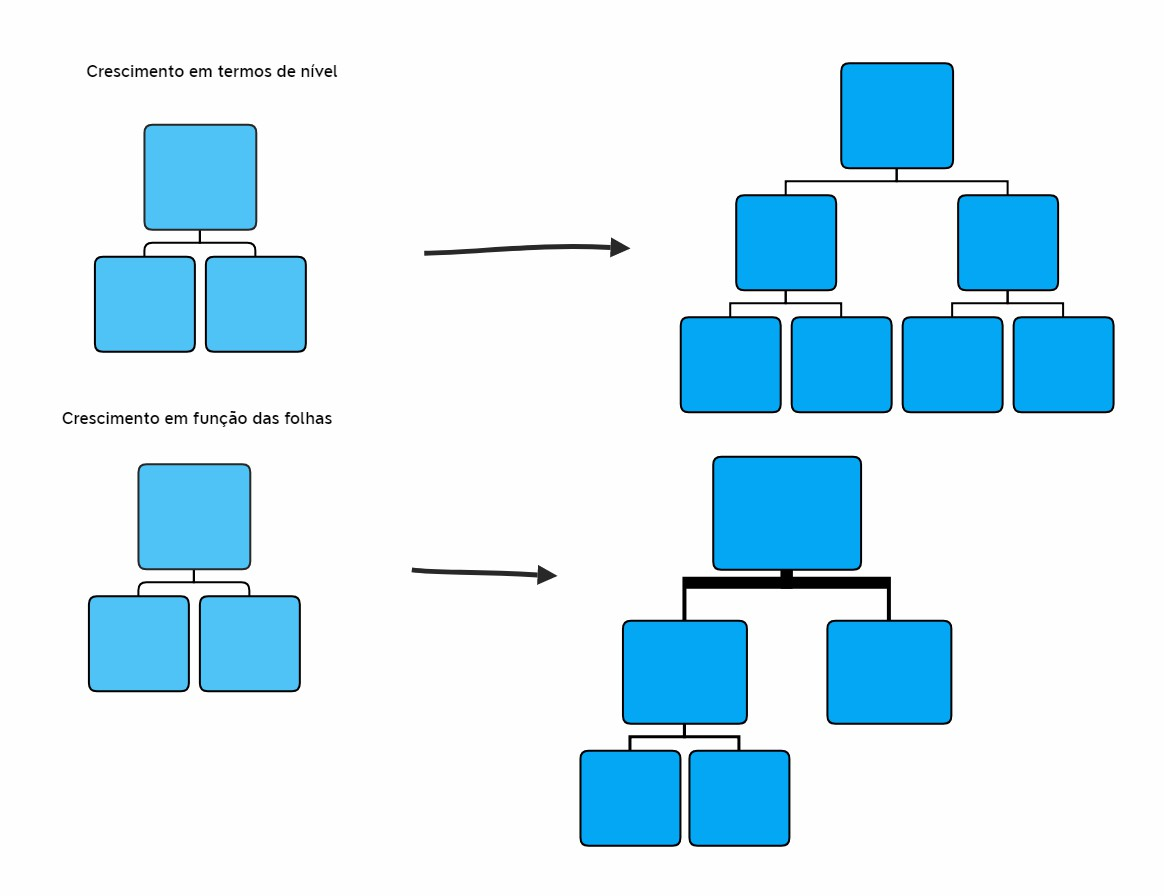
\includegraphics[width=0.7\linewidth]{Modelos/Figuras/xgboost}
	
	Fonte: Adaptação de \citeonline{korstanje2021}
\end{figure}


Na Figura \ref{fig:xgboost} pode ser visto como cada modelo é ajustado, no crescimento da árvore em folha e em nível.

\begin{figure}[H]
	\centering
	\caption{XGBoost e LigthGBM regressão}\label{fig:1-xgb-regressao}
	\includegraphics[width=0.7\linewidth]{Modelos/Figuras/0-xgb-regressão}
	
\end{figure}

\begin{figure}[H]
	\centering
	\includegraphics[width=0.7\linewidth]{Modelos/Figuras/0-lgbm-regressão}	
	
	
	Fonte: Elaboração própria a partir de dados da SANEPAR (2018 a 2020)
	
\end{figure}

Na Figura \ref{fig:1-xgb-regressao} é um modelo baseado nos dados coletados da SANEPAR.

